\documentclass[letterpaper,12pt]{article}

% --- Packages
%\usepackage[paperwidth=5.5in, paperheight=4.25in,margin=0in]{geometry}

\usepackage{tikz} 			%draw

\usepackage{fontspec}		%Set font
\setmainfont{Orbit}         % special by Evan Pittson Design

\usepackage{ifthen}			% if then else

% --- Formatting
\pagenumbering{gobble}


% --- Defined Values
% Constants
\newcommand{\altMargin}{1}
%\newcommand{\cardHeight}{4.25}
%\newcommand{\cardWidth}{5.5}
\newcommand{\lrMarginStart}{2.7}
\newcommand{\udMarginStart}{2.2}
\newcommand{\senderNAnchor}{1.7}
\newcommand{\recipientSAnchor}{-1.9}
\newcommand{\sender}{Sender}
\newcommand{\recipient}{Recipient}
% Set Specific Variables
\newcommand{\setNumber}{0}
\newcommand{\cardNumber}{1}
\newcommand{\cardTitle}{title goes here}
\newcommand{\senderOn}{0}
\newcommand{\recipientOn}{0}
\newcommand{\qrkNumSty}{QRK$\;$M$7_{\setNumber}\;20200530:\cardNumber/20\smile\setNumber/20\;$T$9$ }
% Styling
\newcommand{ \cardTitleSty }[1]{\raggedright \large \MakeUppercase #1}
\newcommand{ \personSty }[1]{\raggedright \normalsize \MakeUppercase #1}
% Instructions
\newcommand{\single}[1]{#1}							
\newcommand{\double}[2]{#1,#2}
\newcommand{\triple}[3]{#1,#2,3}
\newcommand{\singleSingle}[2]{#1,#2}
\newcommand{\doubleSingle}[3]{#1,#2,#3}
\newcommand{\tripleSingle}[4]{#1,#2,#3,#4}
\newcommand{\singleDouble}[3]{#1,#2,#3}
\newcommand{\doubleDouble}[4]{#1,#2,#3,#4}
\newcommand{\tripleDouble}[5]{#1,#2,#3,#4,#5}
\newcommand{\singleTriple}[4]{#1,#2,#3,#4}
\newcommand{\doubleTriple}[5]{#1,#2,#3,#4,#5}
\newcommand{\tripleTriple}[6]{#1,#2,#3,#4,#5,#6}



\begin{document}

\begin{figure}
%\resizebox{5.5in}{4.25in}
%	{
	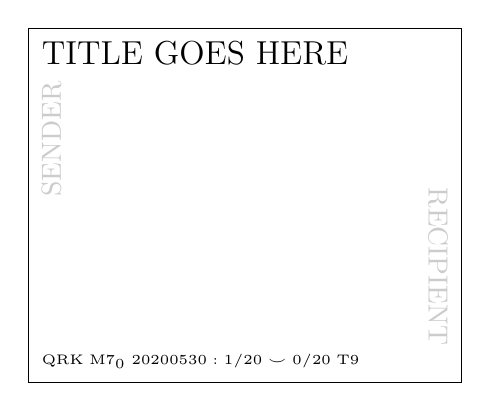
\begin{tikzpicture}[]
		
		% card
    	\draw (-2.75,-2.25) rectangle (2.75, 2.25);
    	
    	% title
    	\node[anchor=north west] at (-\lrMarginStart,\udMarginStart) { \cardTitleSty{\cardTitle}};
    	
    	% QRK Number
    	\node[anchor=south west] at (-\lrMarginStart, -\udMarginStart) { \tiny \qrkNumSty};

    	% sender label 
    	\ifthenelse{\senderOn = 1}
    					 % for the sender
    					 {\node[anchor=north east, rotate = 90] at (-\lrMarginStart,\senderNAnchor) {\personSty{\sender}};}
    					 % not for sender
    					 {\node[anchor=north east, rotate = 90, text = black!20!white] at (-\lrMarginStart,\senderNAnchor) {\personSty{\sender}};} 

    	% recipient label 
    	\ifthenelse{\recipientOn = 1}
    					 % for the recipient
    					 {\node[anchor=north east, rotate = -90 ] at (\lrMarginStart, \recipientSAnchor) {\personSty{\recipient}};}
    					 % not for recipient
    					 {\node[anchor=north east, rotate = -90, text = black!20!white ] at (\lrMarginStart,\recipientSAnchor) {\personSty{\recipient}};} 
		
	\end{tikzpicture}

\end{figure}

\end{document}